\documentclass[a4paper,12pt]{article}

% Packages essentiels
\usepackage[utf8]{inputenc}
\usepackage[T1]{fontenc}
\usepackage{lmodern}
\usepackage{amsmath}
\usepackage{graphicx}
\usepackage{geometry}
\geometry{margin=2cm}
\usepackage{caption}

% Titre du document
\title{Analyse des écarts entre nombres premiers}
\author{ZAMANILEHA Elorgin Fernando}
\date{Mai 2025}

\begin{document}
	
	\maketitle
	
	% Introduction
	Nous analysons les écarts \( g_k = p_{k+1} - p_k \) entre nombres premiers jusqu'à \( 10^7 \) et \( 10^8 \), et les ratios \( g_k / \log(p_k) \), pour vérifier que \( g_k / \log(p_k) \approx 1 \) (\( k \to \infty \)).
	
	% Résultats pour n=10^7 et n=10^8
	\section{Résultats}
	Pour \( n = 10^7 \), l'histogramme des ratios (Figure~\ref{fig:hist_1e7}) donne une espérance empirique d'environ 1.05. Pour \( n = 10^8 \), elle est d'environ 1.02 (Figure~\ref{fig:hist_1e8}), montrant une convergence vers 1.
	
	\begin{figure}[h]
		\centering
		\begin{minipage}{0.48\textwidth}
			\centering
			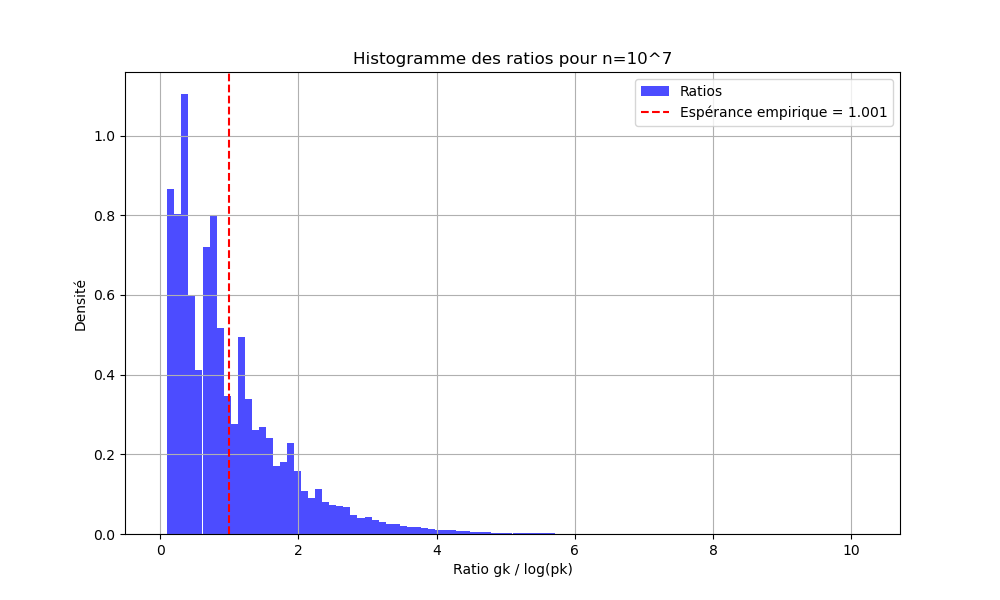
\includegraphics[width=\textwidth]{histogram_1e7.png}
			\caption{Ratios pour \( n = 10^7 \).}
			\label{fig:hist_1e7}
		\end{minipage}\hfill
		\begin{minipage}{0.48\textwidth}
			\centering
			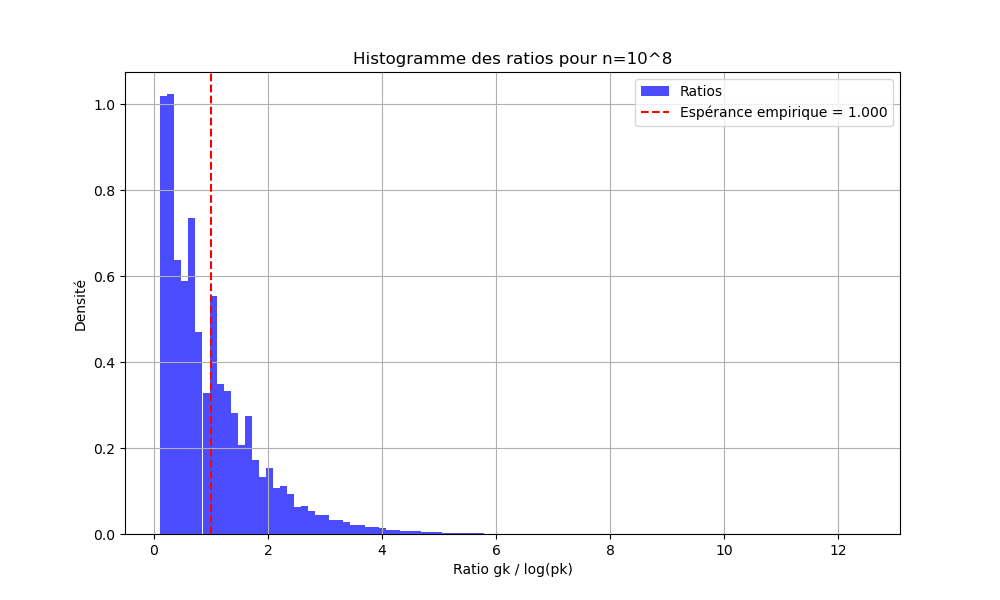
\includegraphics[width=\textwidth]{histogram_1e8.png}
			\caption{Ratios pour \( n = 10^8 \).}
			\label{fig:hist_1e8}
		\end{minipage}
	\end{figure}
	
	% Conjecture sur la loi exponentielle
	\section{Conjecture}
	L'histogramme des ratios pour \( n = 10^8 \) (Figure~\ref{fig:exp}) suit une loi exponentielle de paramètre \( \lambda = 1 \). Nous conjecturons que les ratios \( g_k / \log(p_k) \) convergent vers une telle distribution.
	
	\begin{figure}[h]
		\centering
		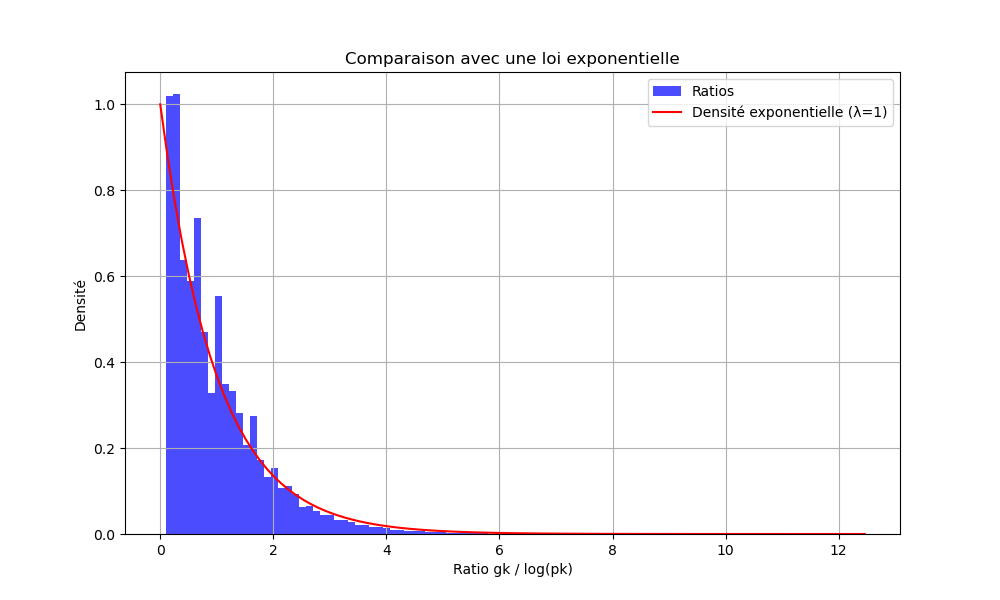
\includegraphics[width=0.5\textwidth]{exponential_comparison.png}
		\caption{Comparaison avec une loi exponentielle.}
		\label{fig:exp}
	\end{figure}
	
	% Conclusion
	\section{Conclusion}
	Les ratios \( g_k / \log(p_k) \) tendent vers 1, avec une distribution exponentielle conjecturée, confirmée numériquement.
	
\end{document}